\documentclass[11pt]{jarticle}

\usepackage[dvipdfmx]{graphicx}

\setlength{\oddsidemargin}{-6.35mm}
\setlength{\textwidth}{171.9mm}

\begin{document}

\title{画像処理実験 第1回}
\author{09430509\\今田将也}
\date{\number\year 年\number\month 月\number\day 日}
\maketitle

\section{課題1}

\subsection{配列の数値を書き換え}

\begin{figure}[htbp]
    \begin{tabular}{ccc}
        \begin{minipage}{0.33\hsize}
            \begin{center}
                
\includegraphics[scale=.5]{1-1.png}
                \caption{1-1の画像}
            \end{center}
        \end{minipage}
        \begin{minipage}{0.33\hsize}
            \begin{center}
                
\includegraphics[scale=.5]{1-2.png}
                \caption{1-2の画像}
            \end{center}
        \end{minipage}
        \begin{minipage}{0.33\hsize}
            \begin{center}
                
\includegraphics[scale=.5]{1-3.png}
                \caption{1-3の画像}
            \end{center}
        \end{minipage}
    \end{tabular}
\end{figure}

\subsection{Processを書き換えた結果}
\subsubsection{カラー画像から R, G, B への分解}

以下のように,配列dstのp+0要素の赤成分のみを代入することで実装した.
また,p+1要素,p+2要素にsrc[p+0]を代入することで緑成分のみ,青成分のみを取り出した.

\begin{verbatim}
    (プログラム一部省略)
    dst[p+0]=src[p+0];
    dst[p+1]=0;
    dst[p+2]=0;
\end{verbatim}
\begin{figure}[htbp]
    \begin{tabular}{ccc}
        \begin{minipage}{0.33\hsize}
            \begin{center}
                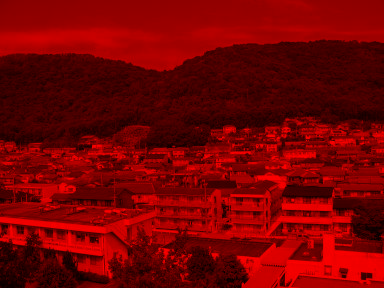
\includegraphics[scale=.3]{1-4.png}
                \caption{赤色の画像}
            \end{center}
        \end{minipage}
        \begin{minipage}{0.33\hsize}
            \begin{center}
                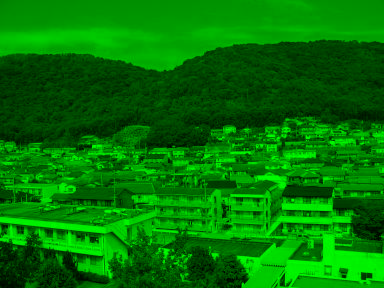
\includegraphics[scale=.3]{1-4-1.png}
                \caption{緑色の画像}
            \end{center}
        \end{minipage}
        \begin{minipage}{0.33\hsize}
            \begin{center}
                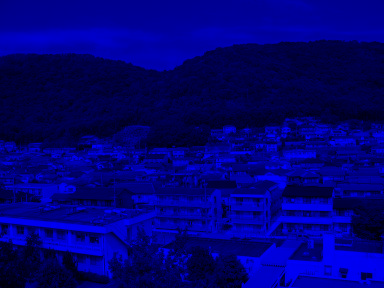
\includegraphics[scale=.3]{1-4-2.png}
                \caption{青色の画像}
            \end{center}
        \end{minipage}
    \end{tabular}
\end{figure}

\subsubsection{画像の拡大}

画像の拡大をするために,画像の色を抽出する手順の前に拡大を行う手順を入れた.
以下はそのソースコードを一部抜粋した.

\begin{verbatim}
    //拡大
    var xx=Math.round(x/4)+200,yy=Math.round(y/4)+100;
    q=(wdt*yy+xx)*4;
    dst[p+0]=src[q+0];
    dst[p+1]=src[q+1];
    dst[p+2]=src[q+2];

    //色の抽出
    p=(y*wdt+x)*4;
    dst[p+0]=r/49;
    dst[p+1]=g/49;
    dst[p+2]=b/49;
    dst[p+3]=255;
\end{verbatim}
\begin{figure}[h]
    \centering
    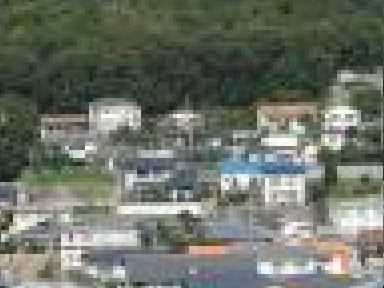
\includegraphics[scale=.3]{1-4-3.png}
    \caption{4倍に拡大した画像}
\end{figure}

\subsection{1-5}
\subsubsection{C言語で画像処理}
講義のページにあるimage.h,image.c,image2.c,image2.cxxを利用し,
easyProcess.cを作成後以下のコマンドにて実行をおこなった.

\begin{verbatim}
    $ gcc --no-warnings -O easyProcess.c image.c image2.c
    $ ./a.out 0.jpg a.jpg
\end{verbatim}

生成された画像を図\ref{a.jpg}に示した.
\begin{figure}[htbp]
    \centering
    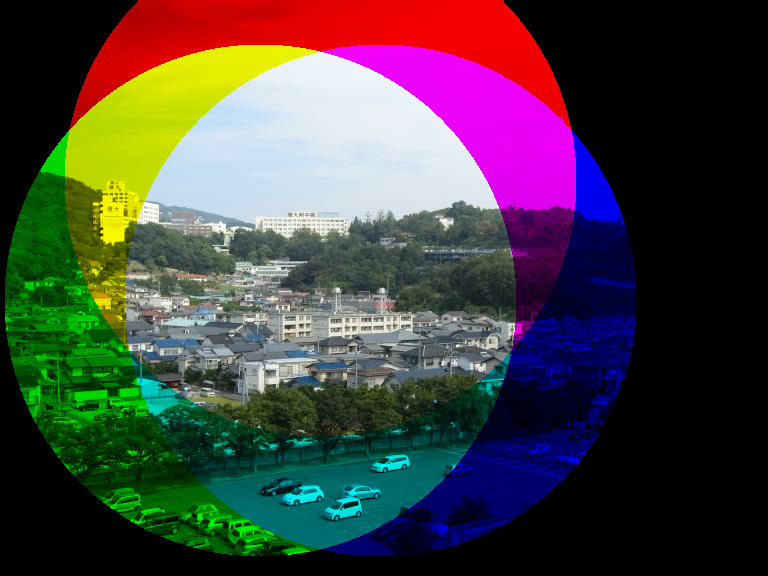
\includegraphics[scale=.2]{a.jpg}
    \caption{easyProcessにて生成された画像}
    \label{a.jpg}
\end{figure}

\subsubsection{赤色のみ抽出}
IElem(dst,x,y,0)にIElem(src,x,y,0)で赤要素のみを入れた.緑と青に関しては,
例のように0を入れるつまり無視すれば良いので,コメントアウトすることで実装した.
図\ref{red.jpg}に示す

\begin{figure}[htbp]
    \centering
    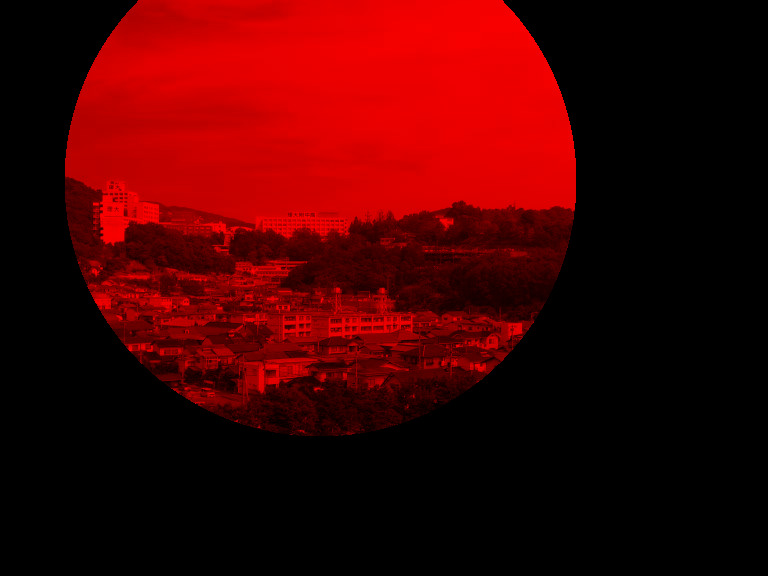
\includegraphics[scale=.2]{red.jpg}
    \caption{赤色のみ抽出した画像}
    \label{red.jpg}
\end{figure}

\subsubsection{緑色のみ抽出}
赤色のときと同様の方法で実装した.
図\ref{b.jpg}に示す

\begin{figure}[htbp]
    \centering
    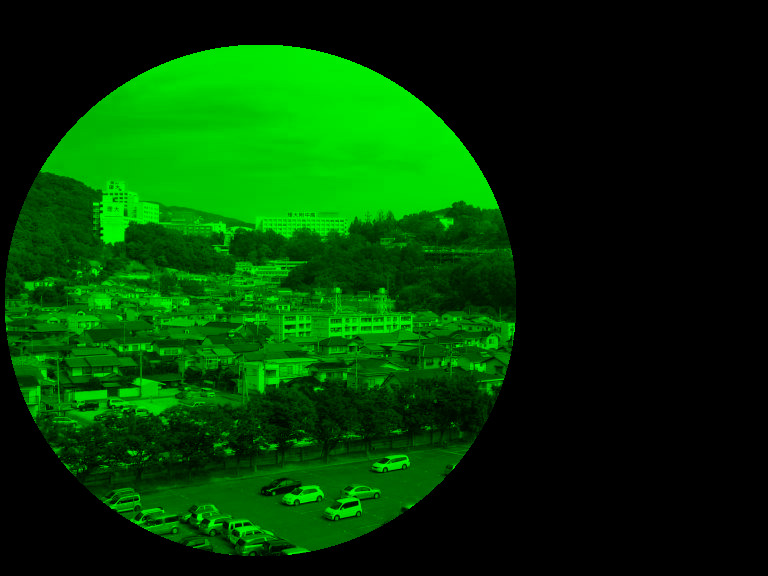
\includegraphics[scale=.2]{b.jpg}
    \caption{緑色のみ抽出した画像}
    \label{b.jpg}
\end{figure}

\subsubsection{青色のみ抽出}
赤色のときと同様の方法で実装した.
図\ref{c.jpg}に示す

\begin{figure}[htbp]
    \centering
    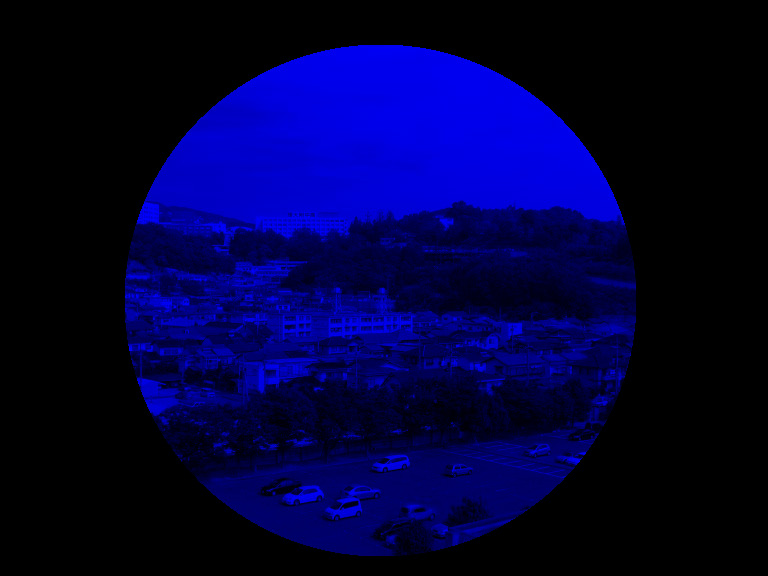
\includegraphics[scale=.2]{c.jpg}
    \caption{青色のみ抽出した画像}
    \label{c.jpg}
\end{figure}

\subsubsection{画像の拡大}
画像の拡大は,IElemのsrcで指定されている箇所のxとyをそれぞれ変更することで
拡大の実装ができる.以下そのコードを一部抜粋したものである
\begin{verbatim}
    int qx = round((x)/2);
    int qy = round((y)/2); 
    IElem(dst,x,y,0) = IElem(src,qx,qy,0)*disk(x,y,320,180)/256; // red at (x,y)
\end{verbatim}
また,その結果の画像を図\ref{kakudai.jpg}に示す.
\begin{figure}[htbp]
    \centering
    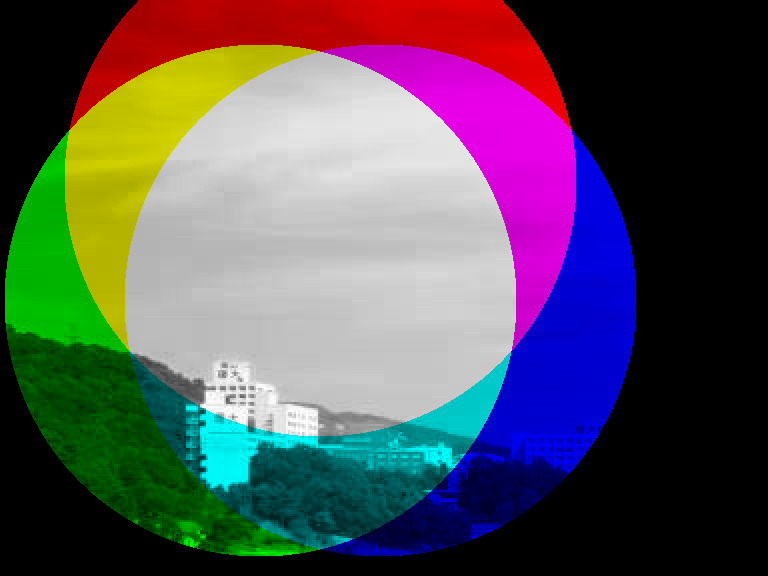
\includegraphics[scale=.2]{kakudai.jpg}
    \caption{拡大した画像}
    \label{kakudai.jpg}
\end{figure}

\subsubsection{スマホで撮影した画像での実験}
実験元の画像を図\ref{196585.jpg}に示す.
\begin{figure}[htbp]
    \centering
    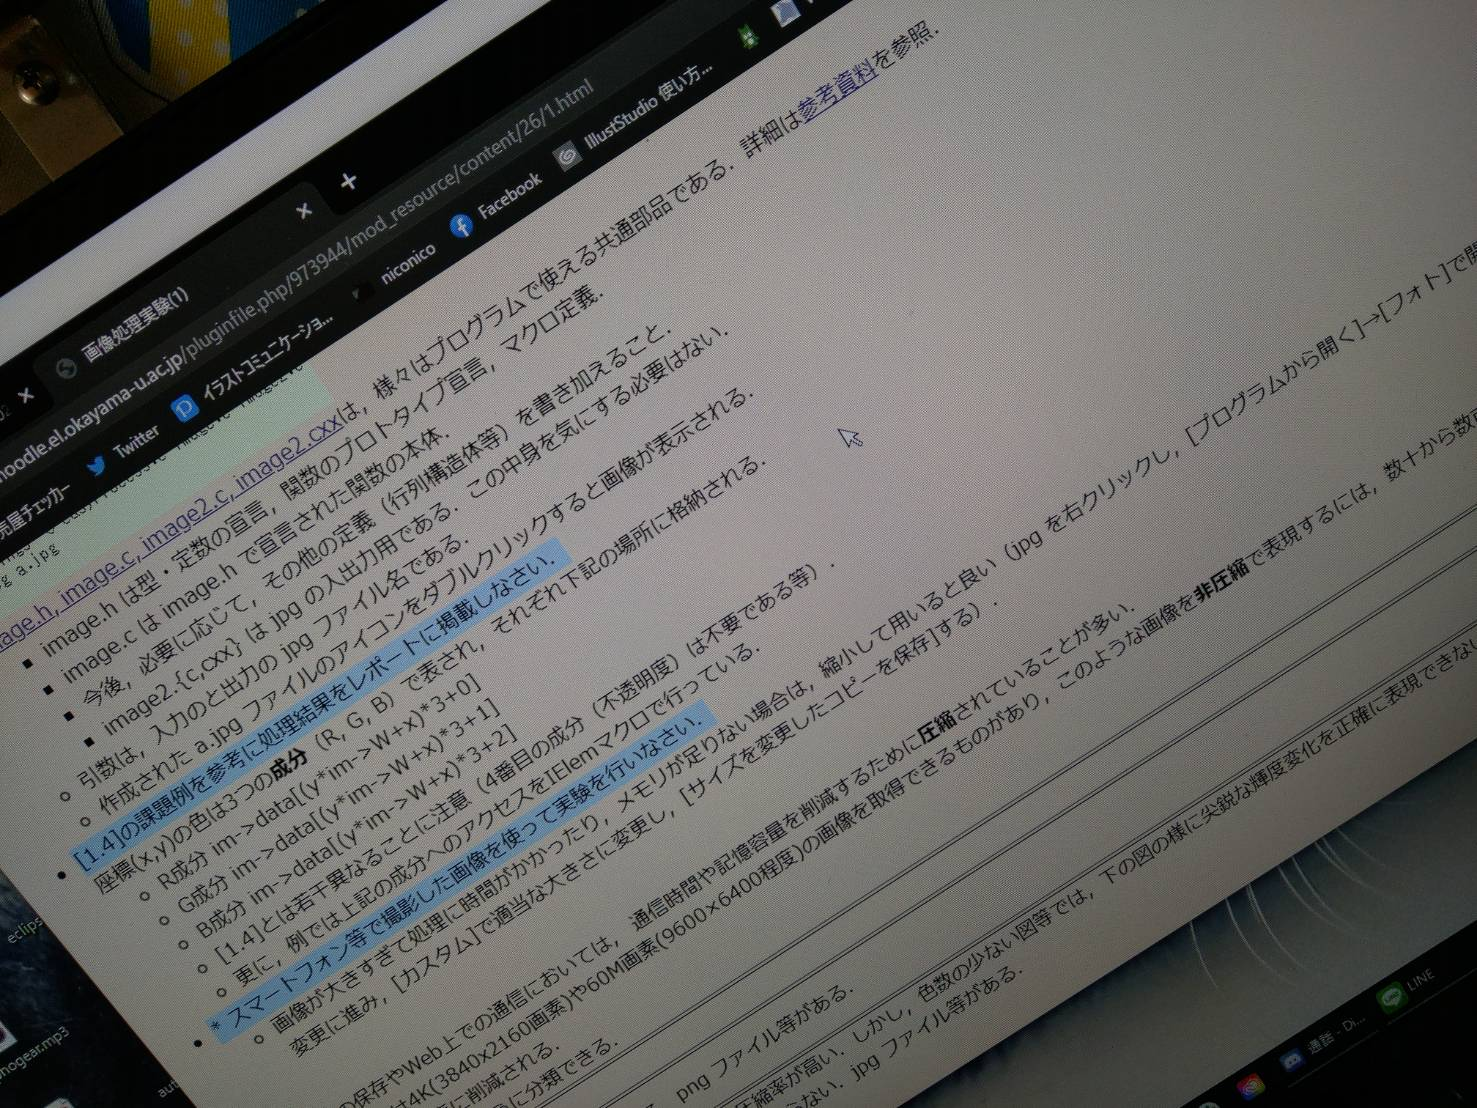
\includegraphics[scale=.1]{196585.jpg}
    \caption{スマホで撮影した画像}
    \label{196585.jpg}
\end{figure}

easyProcessを実行した結果を図\ref{a3.jpg}に示す.
\begin{figure}[htbp]
    \centering
    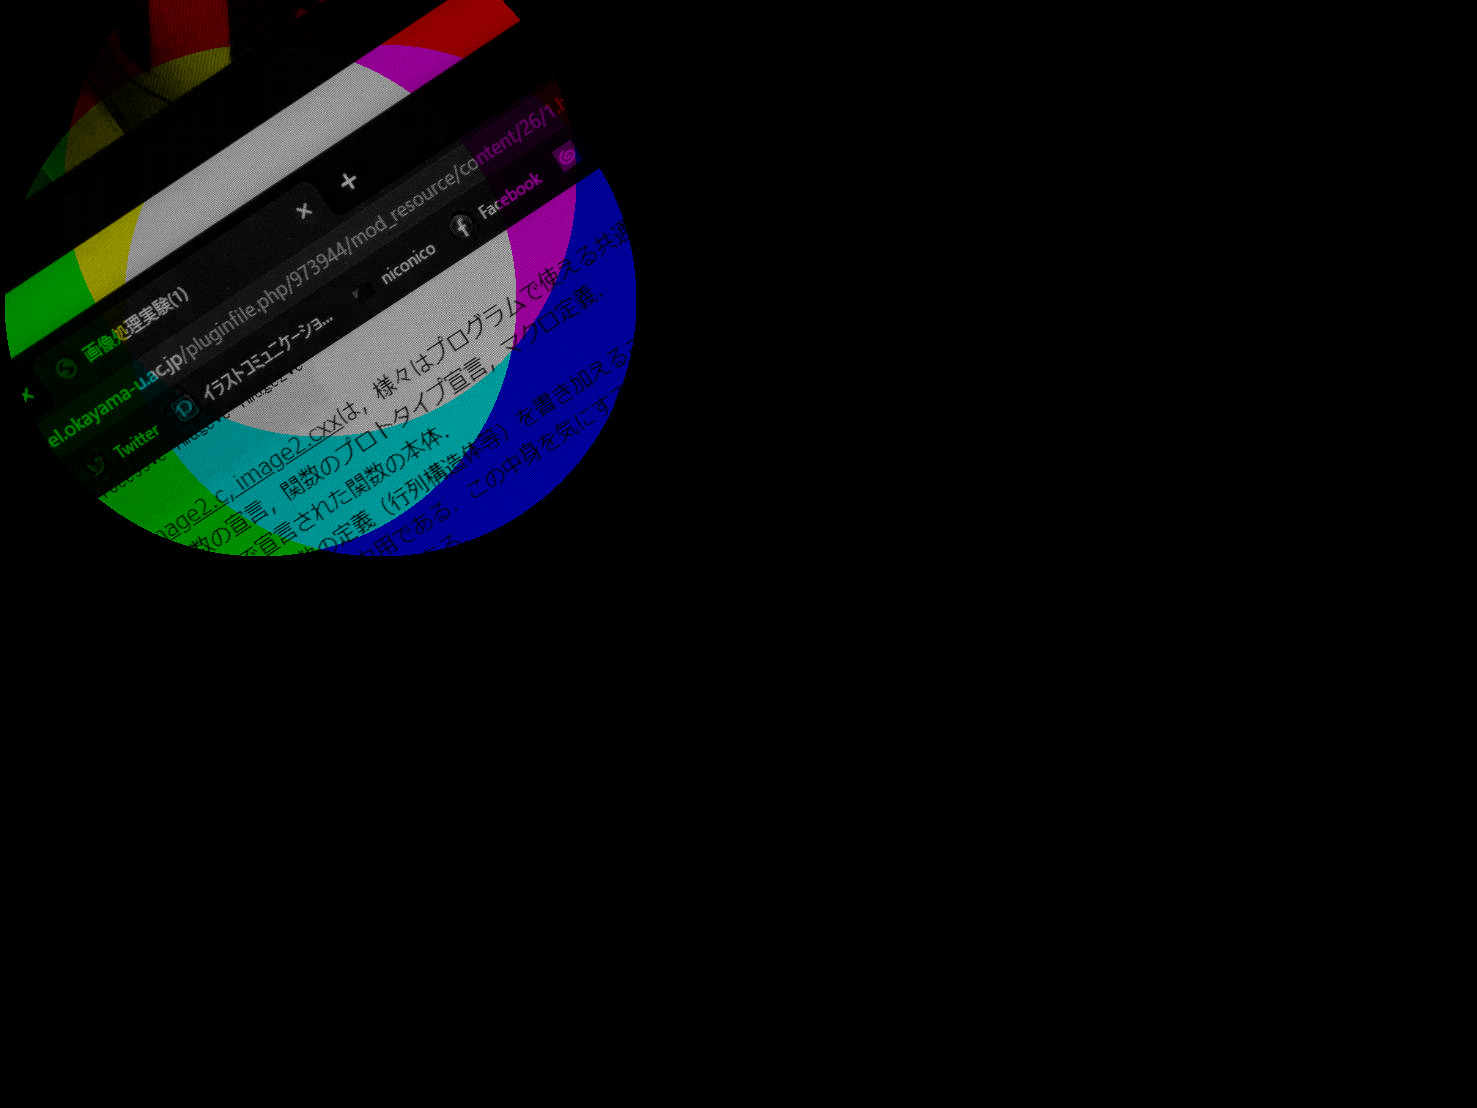
\includegraphics[scale=.1]{a3.jpg}
    \caption{easyProcessを実行した結果}
    \label{a3.jpg}
\end{figure}

なお,拡大についても実験を行った.その結果は図\ref{sumaho_kakudai.jpg}に示した.
\begin{figure}[htbp]
    \centering
    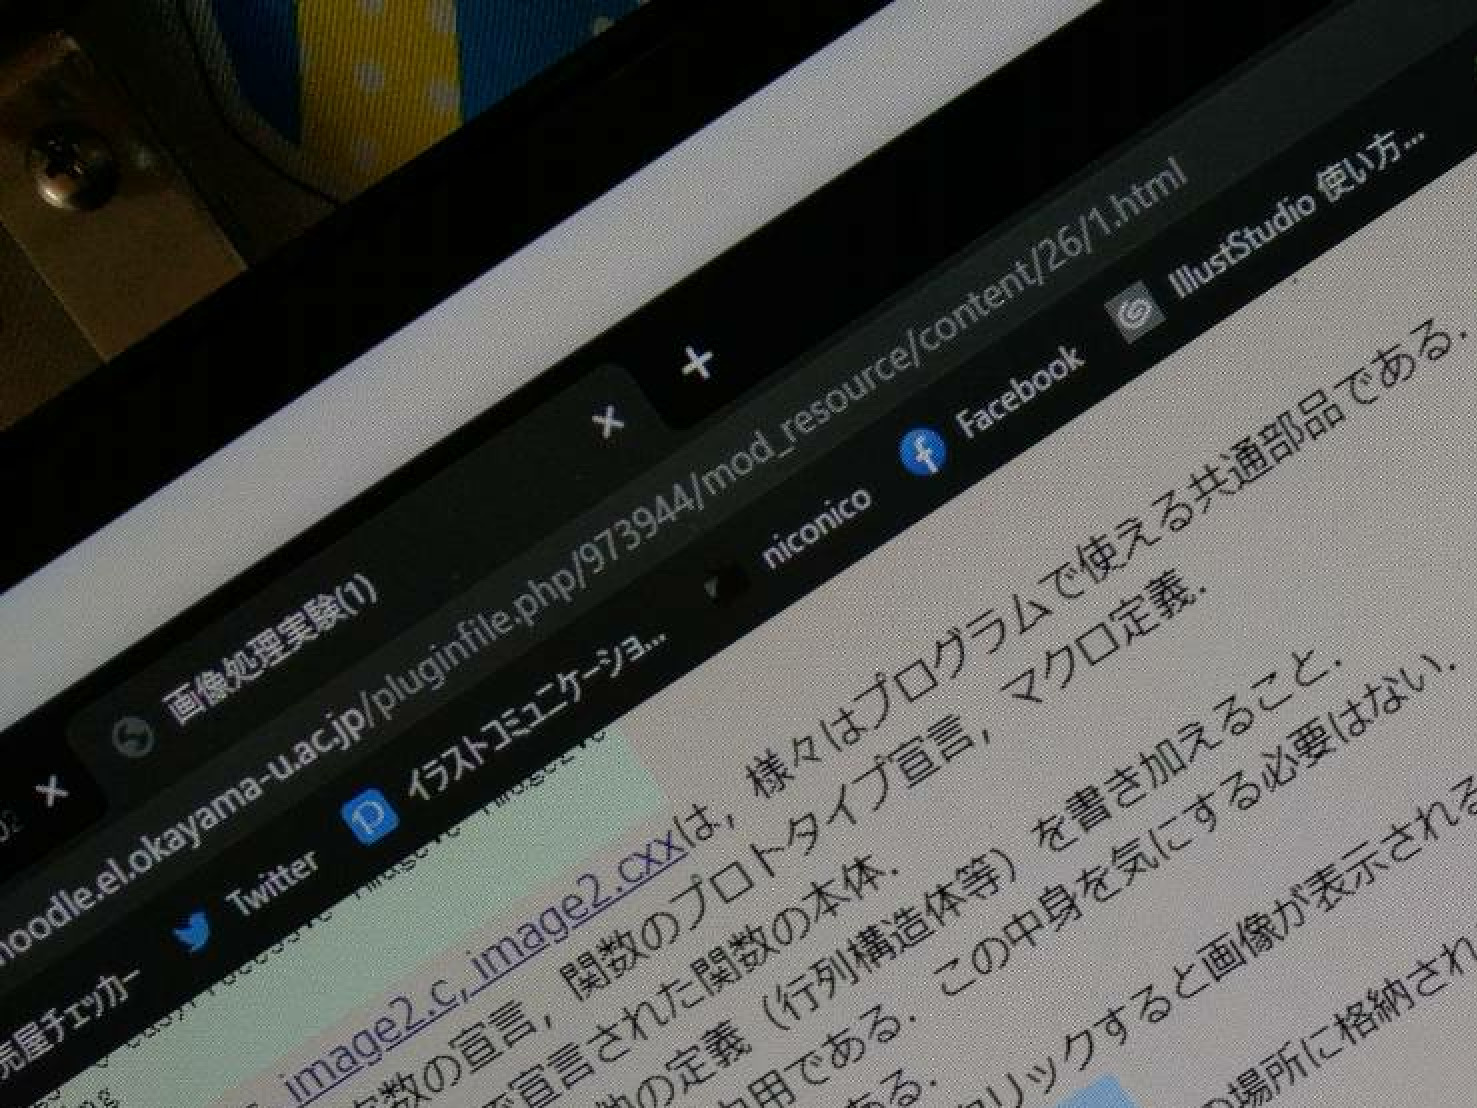
\includegraphics[scale=.1]{sumaho_kakudai.jpg}
    \caption{スマホで撮影した画像を拡大した結果}
    \label{sumaho_kakudai.jpg}
\end{figure}

\subsection{様々な型式でのファイルサイズ(および画質)を比較}

元形式がjpg形式の画像を用いて,png,gif,bmp,webpについてそれぞれ比較を行った.
画像の縦幅,横幅に変化はなく,純粋にファイルの書き出し形式のみ変更を行った.
\begin{table}[h]
    \begin{center}
    \begin{tabular}{l|llll}
    \cline{1-2}
    形式        & ファイルサイズ(B) &  &  &  \\ \cline{1-2}
    .jpg(元画像) & 7,692,612  &  &  &  \\
    .png      & 29,699,714 &  &  &  \\
    .gif      & 13,502,072 &  &  &  \\
    .bmp      & 36,578,442 &  &  &  \\
    .webp     & 7,192,510  &  &  &  \\ \cline{1-2}
    \end{tabular}
\end{center}
\end{table}

無圧縮であるWindows独自規格のbmpファイルについて見てみると,やはりファイルサイズは大きくなっている.
また,次いで可逆圧縮形式のpngのファイルサイズも大きくなっていた.Webなどではかなり使われている形式のため,
小さくなるかと思っていたがそうではなかった.
そして同様の可逆圧縮のgifはpngほど大きくはないが,それでも元画像の約2倍程度にまでファイルサイズは大きくなっている.
最後に,非可逆圧縮,可逆圧縮の両方を扱えるwebpについてだが,ここでは可逆圧縮で実験を行った.結果,jpgよりも500KB,
非可逆圧縮の実験については,今回は行わなかった.

\section{感想}
数値からできているという画像のなり立ちについて理解をすることができた.
また,加法混色で様々な色が表現され,その要素となる赤,緑,青をそれぞれ抽出するという
基礎的な画像処理の手順についてもC言語を通して少しだけ理解をすることができ満足した.
しかし,深い部分の処理について触れてはいないため,今後の実験を通しそこを理解することを
目標に今期の実験に取り組みたい.

\end{document}